% Capitolul 8: Extensii Moderne ale Seriilor de Timp
% Prezentare academică de calitate Harvard
% Program de licență, Academia de Studii Economice din București

\documentclass[9pt, aspectratio=169, t]{beamer}

% Asigură încadrarea conținutului pe diapozitive
\setbeamersize{text margin left=8mm, text margin right=8mm}

%=============================================================================
% CONFIGURARE TEMĂ ȘI STIL
%=============================================================================
\usetheme{default}
% Using default theme for clean header/footer control

% Color Palette (matching Redispatch PDF)
\definecolor{MainBlue}{RGB}{26, 58, 110}
\definecolor{AccentBlue}{RGB}{26, 58, 110}
\definecolor{IDAred}{RGB}{205, 0, 0}
\definecolor{DarkGray}{RGB}{51, 51, 51}
\definecolor{MediumGray}{RGB}{128, 128, 128}
\definecolor{LightGray}{RGB}{248, 248, 248}
\definecolor{VeryLightGray}{RGB}{235, 235, 235}
\definecolor{KeynoteGray}{RGB}{218, 218, 218}
\definecolor{SectionGray}{RGB}{120, 120, 120}
\definecolor{FooterGray}{RGB}{100, 100, 100}
\definecolor{Crimson}{RGB}{220, 53, 69}
\definecolor{Forest}{RGB}{46, 125, 50}
\definecolor{Amber}{RGB}{181, 133, 63}
\definecolor{Orange}{RGB}{230, 126, 34}
\definecolor{Purple}{RGB}{142, 68, 173}

% Gradient background (exact Keynote 315° gradient: white to RGB 218,218,218)
\setbeamertemplate{background}{%
    \begin{tikzpicture}[remember picture, overlay]
        \shade[shading=axis, shading angle=315,
        top color=white, bottom color=KeynoteGray]
        (current page.south west) rectangle (current page.north east);
    \end{tikzpicture}%
}
% Fallback solid color for compatibility
\setbeamercolor{background canvas}{bg=}

\setbeamercolor{palette primary}{bg=MainBlue, fg=white}
\setbeamercolor{palette secondary}{bg=MainBlue!85, fg=white}
\setbeamercolor{palette tertiary}{bg=MainBlue!70, fg=white}
\setbeamercolor{structure}{fg=MainBlue}
\setbeamercolor{title}{fg=IDAred}
\setbeamercolor{frametitle}{fg=IDAred, bg=}
\setbeamercolor{block title}{bg=MainBlue, fg=white}
\setbeamercolor{block body}{bg=VeryLightGray, fg=DarkGray}
\setbeamercolor{block title alerted}{bg=Crimson, fg=white}
\setbeamercolor{block body alerted}{bg=Crimson!8, fg=DarkGray}
\setbeamercolor{block title example}{bg=Forest, fg=white}
\setbeamercolor{block body example}{bg=Forest!8, fg=DarkGray}
\setbeamercolor{item}{fg=MainBlue}

% Footer colors (override Madrid theme blue)
\setbeamercolor{author in head/foot}{fg=FooterGray, bg=}
\setbeamercolor{title in head/foot}{fg=FooterGray, bg=}
\setbeamercolor{date in head/foot}{fg=FooterGray, bg=}
\setbeamercolor{section in head/foot}{fg=FooterGray, bg=}
\setbeamercolor{subsection in head/foot}{fg=FooterGray, bg=}

% Bullet styles (apply everywhere including blocks)
\setbeamertemplate{itemize item}{\color{MainBlue}$\boxdot$}
\setbeamertemplate{itemize subitem}{\color{MainBlue}$\blacktriangleright$}
\setbeamertemplate{itemize subsubitem}{\color{MainBlue}\tiny$\bullet$}
\setbeamertemplate{itemize/enumerate body begin}{\normalsize}
\setbeamertemplate{itemize/enumerate subbody begin}{\normalsize}

% Item spacing - compact style
\setlength{\leftmargini}{10pt}       % Level 1: minimal indent
\setlength{\leftmarginii}{10pt}      % Level 2: minimal additional indent
% Compact list spacing (zero extra space before/after lists in blocks)
\makeatletter
\def\@listi{\leftmargin\leftmargini \topsep 0pt \parsep 0pt \itemsep 0pt}
\def\@listii{\leftmargin\leftmarginii \topsep 0pt \parsep 0pt \itemsep 0pt}
\makeatother

\setbeamertemplate{navigation symbols}{}

%=============================================================================
% CUSTOM HEADLINE
%=============================================================================
\setbeamertemplate{headline}{%
    \vskip10pt%
    \hbox to \paperwidth{%
        \hskip0.5cm%
        {\small\color{FooterGray}\renewcommand{\hyperlink}[2]{##2}\insertsectionhead}%
        \hfill%
        \textcolor{FooterGray}{\small\insertframenumber}%
        \hskip0.5cm%
    }%
    \vskip4pt%
    {\color{FooterGray}\hrule height 0.4pt}%
}

%=============================================================================
% CUSTOM FOOTER
%=============================================================================
\usepackage{fontawesome5}

\setbeamertemplate{footline}{%
    {\color{FooterGray}\hrule height 0.4pt}%
    \vskip4pt%
    \hbox to \paperwidth{%
        \hskip0.5cm%
        \textcolor{FooterGray}{\small Analiza și Prognoza Seriilor de Timp}%
        \hfill%
        \raisebox{-0.1em}{%
            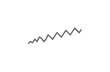
\begin{tikzpicture}[x=0.08em, y=0.08em, line width=0.4pt]
                \draw[FooterGray] (0,3) -- (1,4) -- (2,3.5) -- (3,5) -- (4,4) -- (5,6) -- (6,5.5) -- (7,4) -- (8,5) -- (9,7) -- (10,6) -- (11,5) -- (12,6.5) -- (13,8) -- (14,7) -- (15,6) -- (16,7.5) -- (17,9) -- (18,8) -- (19,7) -- (20,8.5) -- (21,10) -- (22,9) -- (23,8) -- (24,9.5);
            \end{tikzpicture}%
        }%
        \hskip0.5cm%
    }%
    \vskip6pt%
}

%=============================================================================
% PACHETE
%=============================================================================
\usepackage[utf8]{inputenc}
\usepackage[T1]{fontenc}
\usepackage{amsmath, amssymb, amsthm}
\usepackage{mathtools}
\usepackage{bm}
\usepackage{tikz}
\usetikzlibrary{arrows.meta, positioning, shapes, calc, decorations.pathreplacing, shadings}
\usepackage{booktabs}
\usepackage{multirow}
\usepackage{array}
\usepackage{graphicx}
\usepackage{hyperref}
\usepackage{colortbl}
\hypersetup{colorlinks=true, linkcolor=MainBlue, urlcolor=MainBlue}
\graphicspath{{../../logos/}{../../charts/}}
\hfuzz=2pt  % Suppress tiny overfull warnings (<2pt)
\vfuzz=2pt  % Suppress tiny vertical overfull warnings (<2pt)

%=============================================================================
% COMANDA QUANTLET
%=============================================================================
\newcommand{\quantlet}[2]{%
    \hfill\href{#2}{%
        \raisebox{-0.15em}{\includegraphics[height=0.7em]{ql_logo.png}}%
        \textcolor{MainBlue}{\tiny\ #1}%
    }%
}

%=============================================================================
% PAGINĂ TITLU PERSONALIZATĂ
%=============================================================================
\defbeamertemplate*{title page}{hybrid}[1][]
{
    \vspace{0.2cm}
    % Logos row - top header (with clickable links)
    \begin{center}
        \href{https://www.ase.ro}{\includegraphics[height=1.0cm]{ase_logo.png}}\hspace{0.3cm}%
        \href{https://theida.net}{\includegraphics[height=1.0cm]{ida_logo.png}}\hspace{0.3cm}%
        \href{https://blockchain-research-center.com}{\includegraphics[height=1.0cm]{brc_logo.png}}\hspace{0.3cm}%
        \href{https://www.ai4efin.ase.ro}{\includegraphics[height=1.0cm]{ai4efin_logo.png}}\hspace{0.3cm}%
        \href{https://ipe.ro/new}{\includegraphics[height=1.0cm]{acad_logo.png}}\hspace{0.3cm}%
        \href{https://www.digital-finance-msca.com}{\includegraphics[height=1.0cm]{msca_logo.png}}%
    \end{center}

    \vspace{0.6cm}

    % Main title with Q logos on sides (with clickable links)
    \begin{center}
        \begin{minipage}{0.1\textwidth}
            \centering
            \href{https://quantlet.com}{\includegraphics[height=1.1cm]{ql_logo.png}}
        \end{minipage}%
        \begin{minipage}{0.78\textwidth}
            \centering
            {\LARGE\bfseries\usebeamercolor[fg]{title}\inserttitle}

            \vspace{0.3cm}

            {\usebeamerfont{subtitle}\usebeamercolor[fg]{title}\insertsubtitle}
        \end{minipage}%
        \begin{minipage}{0.1\textwidth}
            \centering
            \href{https://quantinar.com}{\includegraphics[height=1.1cm]{qr_logo.png}}
        \end{minipage}
    \end{center}

    \vspace{0.6cm}

    % Authors (left aligned)
    \hspace{0.5cm}{\usebeamerfont{author}\insertauthor}

    \vspace{0.3cm}

    % Institute/Affiliations (left aligned)
    \hspace{0.5cm}\begin{minipage}[t]{0.9\textwidth}
        \raggedright\small\insertinstitute
    \end{minipage}
}

%=============================================================================
% MEDII PENTRU TEOREME
%=============================================================================
\theoremstyle{definition}
\setbeamertemplate{theorems}[numbered]
\newtheorem{defn}{Definiție}
\newtheorem{thm}{Teoremă}
\newtheorem{prop}{Propoziție}
\newtheorem{rmk}{Observație}

%=============================================================================
% COMENZI PERSONALIZATE
%=============================================================================
\newcommand{\E}{\mathbb{E}}
\newcommand{\Var}{\text{Var}}
\newcommand{\Cov}{\text{Cov}}
\newcommand{\Corr}{\text{Corr}}
\newcommand{\R}{\mathbb{R}}
\newcommand{\N}{\mathbb{N}}
\newcommand{\Z}{\mathbb{Z}}
\newcommand{\B}{\mathbf{B}}
\newcommand{\imark}{\textcolor{MainBlue}{\textbullet}}
\newcommand{\RMSE}{\text{RMSE}}
\newcommand{\MAE}{\text{MAE}}
\newcommand{\MAPE}{\text{MAPE}}

%=============================================================================
% INFORMAȚII TITLU
%=============================================================================
\title[Analiza Seriilor de Timp]{Analiza și Prognoza Seriilor de Timp}
\subtitle{Capitolul 8: Extensii Moderne}
\author[D.T. Pele]{Daniel Traian PELE}
\institute{Academia de Studii Economice din București\\
IDA Institute Digital Assets\\
Blockchain Research Center\\
AI4EFin Artificial Intelligence for Energy Finance\\
Academia Română, Institutul de Prognoză Economică\\
MSCA Digital Finance}
\date{}

\begin{document}

% Title page (no header/footer)
{
\setbeamertemplate{headline}{}
\setbeamertemplate{footline}{}
\begin{frame}
    \titlepage
\end{frame}
}

%=============================================================================
% OUTLINE
%=============================================================================
\begin{frame}{Cuprins}
    \vspace{-0.3cm}
    {\small
    \begin{columns}[T]
        \begin{column}{0.48\textwidth}
            \begin{block}{Fundamente}
                \begin{itemize}\setlength{\itemsep}{3pt}
                    \item Motivație
                    \item ARFIMA: Modele cu Memorie lungă
                    \item Random Forest pentru serii de timp
                    \item LSTM: Deep Learning pentru serii de timp
                    \item Comparație și Selecția modelului
                \end{itemize}
            \end{block}
        \end{column}
        \begin{column}{0.48\textwidth}
            \begin{exampleblock}{Aplicații}
                \begin{itemize}\setlength{\itemsep}{3pt}
                    \item Aplicații practice
                    \item Studiu de Caz: Cursul EUR/RON
                    \item Comparație Finală: Toate Metodele
                    \item Exemple cu Date Reale
                    \item Rezumat
                \end{itemize}
            \end{exampleblock}
        \end{column}
    \end{columns}
    }
\end{frame}

%=============================================================================
% LEARNING OBJECTIVES
%=============================================================================
\begin{frame}{Obiective de învățare}
    \begin{block}{La finalul acestui capitol, veți fi capabili să:}
        \begin{enumerate}\setlength{\itemsep}{0pt}
            \item Înțelegeți conceptul de \textbf{memorie lungă} în seriile de timp
            \item Estimați și interpretați modele \textbf{ARFIMA}
            \item Aplicați \textbf{Random Forest} pentru prognoză seriilor de timp
            \item Construiți rețele \textbf{LSTM} pentru serii temporale
            \item Comparăți performanța modelelor clasice vs ML
            \item Alegeți metoda potrivită în funcție de context
            \item Implementați aceste metode în \textbf{Python}
        \end{enumerate}
    \end{block}
\end{frame}

%=============================================================================
\section{Motivație}
%=============================================================================

\begin{frame}{De la modele clasice la machine learning}
    \begin{block}{Limitările Modelelor ARIMA}
        \begin{itemize}\setlength{\itemsep}{0pt}
            \item Presupun \textbf{memorie scurtă}: autocorelațiile scad exponențial
            \item Relații \textbf{liniare} între variabile
            \item Dificultăți cu \textbf{pattern-uri complexe} și neliniare
            \item Necesită \textbf{staționaritate} (prin diferențiere)
        \end{itemize}
    \end{block}

    \vspace{0.2cm}

    \begin{alertblock}{Soluții Moderne}
        \begin{itemize}\setlength{\itemsep}{0pt}
            \item \textbf{ARFIMA}: Captează memoria lungă (autocorelații care scad lent)
            \item \textbf{Random Forest}: Relații neliniare, robustețe la outlieri
            \item \textbf{LSTM}: Pattern-uri secvențiale complexe, dependențe pe termen lung
        \end{itemize}
    \end{alertblock}
\end{frame}

\begin{frame}{Când să folosim fiecare metodă?}
    \begin{center}
    \begin{tabular}{l|c|c|c|c}
        \toprule
        \textbf{Caracteristică} & \textbf{ARIMA} & \textbf{ARFIMA} & \textbf{RF} & \textbf{LSTM} \\
        \midrule
        Memorie lungă & $\times$ & $\checkmark$ & $\checkmark$ & $\checkmark$ \\
        Relații neliniare & $\times$ & $\times$ & $\checkmark$ & $\checkmark$ \\
        Interpretabilitate & $\checkmark$ & $\checkmark$ & $\sim$ & $\times$ \\
        Date puține & $\checkmark$ & $\checkmark$ & $\times$ & $\times$ \\
        Variabile exogene & $\checkmark$ & $\checkmark$ & $\checkmark$ & $\checkmark$ \\
        Incertitudine & $\checkmark$ & $\checkmark$ & $\sim$ & $\times$ \\
        \bottomrule
    \end{tabular}
    \end{center}

    \vspace{0.3cm}

    \begin{exampleblock}{Regula de Aur}
        \begin{itemize}\setlength{\itemsep}{0pt}
            \item Începe \textbf{simplu} (ARIMA), apoi crește complexitatea doar dacă este justificat de date și performanță.
        \end{itemize}
    \end{exampleblock}
\end{frame}

%=============================================================================
\section{ARFIMA: Modele cu Memorie lungă}
%=============================================================================

\begin{frame}{Ce este memoria lungă?}
    \begin{block}{Memorie Scurtă (ARMA)}
        \begin{itemize}\setlength{\itemsep}{0pt}
            \item Autocorelațiile $\rho_k$ scad \textbf{exponențial}: $|\rho_k| \leq C \cdot r^k$, $r < 1$
            \item Efectele șocurilor dispar \textbf{rapid}
            \item Sumă finită: $\sum_{k=0}^{\infty} |\rho_k| < \infty$
        \end{itemize}
    \end{block}

    \vspace{0.2cm}

    \begin{alertblock}{Memorie lungă (ARFIMA)}
        \begin{itemize}\setlength{\itemsep}{0pt}
            \item Autocorelațiile scad \textbf{hiperbolic}: $\rho_k \sim C \cdot k^{2d-1}$
            \item Efectele șocurilor persistă \textbf{mult timp}
            \item Sumă infinită: $\sum_{k=0}^{\infty} |\rho_k| = \infty$ (pentru $d > 0$)
        \end{itemize}
    \end{alertblock}

    \vspace{0.2cm}

    \begin{exampleblock}{Exemple cu Memorie lungă}
        \begin{itemize}\setlength{\itemsep}{0pt}
            \item Volatilitatea piețelor financiare, debite râuri, trafic rețea, inflație
        \end{itemize}
    \end{exampleblock}
\end{frame}

\begin{frame}{Comparație ACF: memorie scurtă vs lungă}
    \vspace{-0.2cm}
    \begin{center}
        \includegraphics[width=0.90\textwidth, height=0.58\textheight, keepaspectratio]{ch8_acf_comparison.pdf}
    \end{center}
    \vspace{-0.3cm}
    {\footnotesize
    \begin{block}{}
        \begin{itemize}\setlength{\itemsep}{0pt}
            \item \textbf{Stânga}: AR(1) $\succ$ autocorelații care scad exponențial (memorie scurtă)
            \item \textbf{Dreapta}: ARFIMA cu $d=0.35$ $\succ$ autocorelații care scad hiperbolic (memorie lungă)
        \end{itemize}
    \end{block}
    }\quantlet{TSA\_ch8\_acf\_comparison}{https://github.com/QuantLet/TSA/tree/main/TSA_ch8/TSA_ch8_acf_comparison}
\end{frame}

\begin{frame}{Modelul ARFIMA(p,d,q)}
    \vspace{-0.3cm}
    {\small
    \begin{defn}[ARFIMA]
        \begin{itemize}\setlength{\itemsep}{0pt}
            \item \textbf{Model}: Un proces $\{Y_t\}$ urmează un model \textbf{ARFIMA(p,d,q)} dacă:
            $\phi(L)(1-L)^d Y_t = \theta(L)\varepsilon_t$
            \item \textbf{Parametru}: $d \in (-0.5, 0.5)$ este parametrul de \textbf{diferențiere fracționară}
        \end{itemize}
    \end{defn}
    }
    \vspace{-0.1cm}
    {\footnotesize
    \begin{block}{Operatorul de Diferențiere Fracționară}
        \begin{itemize}\setlength{\itemsep}{0pt}
            \item $(1-L)^d = \sum_{k=0}^{\infty} \binom{d}{k}(-L)^k = 1 - dL - \frac{d(1-d)}{2!}L^2 - \cdots$
        \end{itemize}
    \end{block}
    }
    \vspace{-0.1cm}
    {\scriptsize
    \begin{block}{Cazuri Particulare}
        \begin{itemize}\setlength{\itemsep}{0pt}
            \item $d = 0$: ARMA standard (memorie scurtă)
            \item $0 < d < 0.5$: Memorie lungă, staționaritate
            \item $d = 0.5$: Limita staționarității
            \item $0.5 \leq d < 1$: Nestaționaritate, dar mean-reverting
            \item $d = 1$: Random walk (ARIMA standard)
        \end{itemize}
    \end{block}
    }
\end{frame}

\begin{frame}{Interpretarea parametrului $d$}
    \begin{center}
    \begin{tabular}{c|l|l}
        \toprule
        \textbf{Valoare $d$} & \textbf{Comportament ACF} & \textbf{Interpretare} \\
        \midrule
        $d = 0$ & Scădere exponențială & Memorie scurtă \\
        $0 < d < 0.5$ & Scădere hiperbolică & Memorie lungă, staționară \\
        $d = 0.5$ & ACF nesumabilă & La limită \\
        $0.5 < d < 1$ & Scădere foarte lentă & Memorie lungă, nestaționară \\
        $d = 1$ & ACF = 1 (constant) & Random walk \\
        \bottomrule
    \end{tabular}
    \end{center}

    \vspace{0.1cm}

    \begin{block}{Parametrul Hurst $H$}
        \begin{itemize}\setlength{\itemsep}{0pt}
            \item \textbf{Relația}: $d = H - 0.5$
            \begin{itemize}\setlength{\itemsep}{0pt}
                \item $H = 0.5$: Mers aleator (fără memorie)
                \item $H > 0.5$: Persistență (trend-following)
                \item $H < 0.5$: Anti-persistență (mean-reverting)
            \end{itemize}
        \end{itemize}
    \end{block}
\end{frame}

\begin{frame}{Efectul parametrului $d$ asupra ACF}
    \begin{center}
        \includegraphics[width=0.95\textwidth, height=0.75\textheight, keepaspectratio]{ch8_arfima_d_effect.pdf}
    \end{center}
    \vspace{-0.2cm}
    {\footnotesize
    \begin{block}{}
        \begin{itemize}\setlength{\itemsep}{0pt}
            \item Cu cât $d$ este mai mare, cu atât autocorelațiile scad mai lent
            \item Pentru $d \to 0.5$, autocorelațiile rămân semnificative chiar și la lag-uri foarte mari
        \end{itemize}
    \end{block}
    }\quantlet{TSA\_ch8\_arfima\_d\_effect}{https://github.com/QuantLet/TSA/tree/main/TSA_ch8/TSA_ch8_arfima_d_effect}
\end{frame}

\begin{frame}{Exponentul Hurst: interpretare vizuală}
    \begin{center}
        \includegraphics[width=0.88\textwidth, height=0.62\textheight, keepaspectratio]{ch8_hurst_interpretation.pdf}
    \end{center}
    \vspace{-0.2cm}
    {\footnotesize
    \begin{block}{}
        \begin{itemize}\setlength{\itemsep}{0pt}
            \item \textbf{H $<$ 0.5}: Serie care revine frecvent la medie (mean-reverting)
            \item \textbf{H = 0.5}: Mers aleator, imprevizibil
            \item \textbf{H $>$ 0.5}: Serie persistentă, tendințele continuă
        \end{itemize}
    \end{block}
    }\quantlet{TSA\_ch8\_hurst\_interpretation}{https://github.com/QuantLet/TSA/tree/main/TSA_ch8/TSA_ch8_hurst_interpretation}
\end{frame}

\begin{frame}{ARIMA vs ARFIMA: comparație simulată}
    \begin{center}
        \includegraphics[width=0.88\textwidth, height=0.62\textheight, keepaspectratio]{ch8_arima_vs_arfima.pdf}
    \end{center}
    \vspace{-0.2cm}
    {\footnotesize
    \begin{block}{}
        \begin{itemize}\setlength{\itemsep}{0pt}
            \item \textbf{ARIMA} (stânga): ACF scade \textbf{exponențial} $\succ$ șocurile sunt ``uitate'' rapid
            \item \textbf{ARFIMA} (dreapta, $d=0.35$): ACF scade \textbf{hiperbolic} $\succ$ șocurile persistă mult timp
        \end{itemize}
    \end{block}
    }\quantlet{TSA\_ch8\_arima\_vs\_arfima}{https://github.com/QuantLet/TSA/tree/main/TSA_ch8/TSA_ch8_arima_vs_arfima}
\end{frame}

\begin{frame}{Exemplu date reale: analiza memoriei lungi EUR/RON}
    \begin{center}
        \includegraphics[width=0.88\textwidth, height=0.62\textheight, keepaspectratio]{ch8_eurron_long_memory.pdf}
    \end{center}
    \vspace{-0.2cm}
    {\footnotesize
    \begin{block}{}
        \begin{itemize}\setlength{\itemsep}{0pt}
            \item \textbf{Randamente} (stânga): $H \approx 0.50$, $d \approx 0$ $\succ$ \textbf{memorie scurtă} (piață eficientă)
            \item \textbf{Randamente pătrate} (dreapta): $H \approx 0.65$, $d \approx 0.15$ $\succ$ \textbf{memorie lungă} în volatilitate
        \end{itemize}
    \end{block}
    }\quantlet{TSA\_ch8\_eurron\_long\_memory}{https://github.com/QuantLet/TSA/tree/main/TSA_ch8/TSA_ch8_eurron_long_memory}
\end{frame}

\begin{frame}{Estimarea parametrului $d$}
    \begin{block}{Metode de estimare}
        \begin{itemize}\setlength{\itemsep}{0pt}
            \item \textbf{GPH (Geweke-Porter-Hudak)}: Regresie în domeniul frecvență
            \begin{itemize}\setlength{\itemsep}{0pt}
                \item $\ln I(\omega_j) = c - d \cdot \ln\bigl(4\sin^2\frac{\omega_j}{2}\bigr) + \varepsilon_j$
            \end{itemize}
            \item \textbf{R/S (Rescaled Range)}: Metoda lui Hurst
            \begin{itemize}\setlength{\itemsep}{0pt}
                \item $\frac{R}{S}(n) \sim c \cdot n^H$
            \end{itemize}
            \item \textbf{MLE (Maximum Likelihood)}: Estimare completă ARFIMA
            \item \textbf{Whittle}: Aproximare eficientă în domeniul frecvență
        \end{itemize}
    \end{block}

    \vspace{0.2cm}

    {\footnotesize
    \begin{exampleblock}{Implementare}
        \begin{itemize}\setlength{\itemsep}{0pt}
            \item În Python: \texttt{arch} package, \texttt{statsmodels.tsa.arima.model.ARIMA} cu \texttt{order=(p,d,q)} unde $d$ poate fi fracționar
        \end{itemize}
    \end{exampleblock}
    }
    \quantlet{TSA\_ch8\_gph\_estimation}{https://github.com/QuantLet/TSA/tree/main/TSA_ch8/TSA_ch8_gph_estimation}
\end{frame}

\begin{frame}{Exemplu ARFIMA în Python}
    \begin{block}{Cod Python}
        \begin{itemize}\setlength{\itemsep}{0pt}
        \item {\footnotesize
        \texttt{from statsmodels.tsa.arima.model import ARIMA}

        \texttt{model = ARIMA(y, order=(1, 0.3, 1))}

        \texttt{results = model.fit()}
        }
        \end{itemize}
    \end{block}

    \vspace{0.2cm}

    \begin{alertblock}{Notă}
        \begin{itemize}\setlength{\itemsep}{0pt}
            \item Estimarea ARFIMA necesită pachete specializate. În practică, se folosește adesea \texttt{arch} sau \texttt{fracdiff} în Python.
        \end{itemize}
    \end{alertblock}
    \quantlet{TSA\_ch8\_arfima\_estimation}{https://github.com/QuantLet/TSA/tree/main/TSA_ch8/TSA_ch8_arfima_estimation}
\end{frame}

\begin{frame}{Exemplu real: memorie lungă în volatilitate}
    \vspace{-0.2cm}
    \begin{center}
        \includegraphics[width=0.90\textwidth, height=0.55\textheight, keepaspectratio]{ch8_volatility_long_memory.pdf}
    \end{center}
    \vspace{-0.3cm}
    {\footnotesize
    \begin{block}{}
        \begin{itemize}\setlength{\itemsep}{0pt}
            \item \textbf{Fapt Stilizat}: Randamentele financiare au memorie scurtă, dar volatilitatea (|randamente|) are memorie lungă
            \item Aceasta este baza modelelor FIGARCH
        \end{itemize}
    \end{block}
    }\quantlet{TSA\_ch8\_volatility\_long\_memory}{https://github.com/QuantLet/TSA/tree/main/TSA_ch8/TSA_ch8_volatility_long_memory}
\end{frame}

%=============================================================================
\section{Random Forest pentru serii de timp}
%=============================================================================

\begin{frame}{Random Forest: concepte de bază}
    \begin{block}{Ce este Random Forest?}
        \begin{itemize}\setlength{\itemsep}{0pt}
            \item \textbf{Ansamblu} de arbori de decizie
            \item Fiecare arbore antrenat pe un \textbf{subset bootstrap} al datelor
            \item La fiecare nod, se selectează \textbf{aleator} un subset de features
            \item Predicția finală = \textbf{media} predicțiilor tuturor arborilor
        \end{itemize}
    \end{block}

    \vspace{0.2cm}

    \begin{exampleblock}{Avantaje pentru serii de timp}
        \begin{itemize}\setlength{\itemsep}{0pt}
            \item Captează \textbf{relații neliniare}
            \item \textbf{Robust} la outlieri și zgomot
            \item Nu necesită \textbf{staționaritate}
            \item Oferă \textbf{importanța features} (interpretabilitate)
            \item Funcționează bine cu \textbf{multe variabile}
        \end{itemize}
    \end{exampleblock}
\end{frame}

\begin{frame}{Pregătirea datelor pentru Random Forest}
    \begin{block}{Feature Engineering pentru serii de timp}
        \begin{enumerate}\setlength{\itemsep}{0pt}
            \item \textbf{Lag features}: $Y_{t-1}, Y_{t-2}, \ldots, Y_{t-p}$
            \item \textbf{Rolling statistics}: medie mobilă, deviație standard
            \item \textbf{Calendar features}: ziua săptămânii, luna, sezon
            \item \textbf{Trend features}: timp, trend pătratic
            \item \textbf{Variabile exogene}: indicători economici, evenimente
        \end{enumerate}
    \end{block}

    \vspace{0.2cm}

    \begin{alertblock}{Atenție: Data Leakage!}
        \begin{itemize}\setlength{\itemsep}{0pt}
            \item Nu folosi informații din viitor în features
            \item Train/test split: \textbf{temporal}, nu aleator!
            \item Rolling statistics: calculează doar pe date \textbf{anterioare}
        \end{itemize}
    \end{alertblock}
\end{frame}

\begin{frame}{Feature engineering: ilustrare}
    \vspace{-0.2cm}
    \begin{center}
        \includegraphics[width=0.90\textwidth, height=0.58\textheight, keepaspectratio]{ch8_feature_engineering.pdf}
    \end{center}
    \vspace{-0.3cm}
    {\footnotesize
    \begin{block}{}
        \begin{itemize}\setlength{\itemsep}{0pt}
            \item Transformăm seria temporală în features: lag-uri, statistici rolling, iar modelul RF învață relațiile dintre acestea și valorile viitoare
        \end{itemize}
    \end{block}
    }\quantlet{TSA\_ch8\_feature\_engineering}{https://github.com/QuantLet/TSA/tree/main/TSA_ch8/TSA_ch8_feature_engineering}
\end{frame}

\begin{frame}{Random Forest: implementare Python}
    \begin{block}{Cod Python}
        \begin{itemize}\setlength{\itemsep}{0pt}
        \item {\footnotesize
        \texttt{from sklearn.ensemble import RandomForestRegressor}

        \texttt{rf = RandomForestRegressor(n\_estimators=100, max\_depth=10)}

        \texttt{rf.fit(X\_train, y\_train)}

        \texttt{predictions = rf.predict(X\_test)}
        }
        \end{itemize}
    \end{block}
\end{frame}

\begin{frame}{Importanța features și interpretare}
    \begin{block}{Feature Importance}
        \begin{itemize}\setlength{\itemsep}{0pt}
            \item \textbf{Mean Decrease Impurity (MDI)}: Reducerea impurității la fiecare split
            \item \textbf{Permutation Importance}: Cât scade performanța când feature-ul e permutat aleator
        \end{itemize}
    \end{block}

    \vspace{0.2cm}

    \begin{exampleblock}{Interpretare Tipică pentru serii de timp}
        \begin{itemize}\setlength{\itemsep}{0pt}
            \item \texttt{lag\_1} foarte important $\succ$ Autocorelare puternică
            \item \texttt{rolling\_mean} important $\succ$ Trend local contează
            \item \texttt{month} important $\succ$ Sezonalitate prezentă
        \end{itemize}
    \end{exampleblock}

    \vspace{0.2cm}

    {\footnotesize
    \begin{block}{Cod}
        \begin{itemize}\setlength{\itemsep}{0pt}
            \item \texttt{rf.feature\_importances\_} sau \texttt{permutation\_importance(rf, X\_test, y\_test)}
        \end{itemize}
    \end{block}
    }
\end{frame}

\begin{frame}{Random Forest: exemplu de prognoză}
    \vspace{-0.2cm}
    \begin{center}
        \includegraphics[width=0.90\textwidth, height=0.55\textheight, keepaspectratio]{ch8_rf_prediction.pdf}
    \end{center}
    \vspace{-0.3cm}
    {\footnotesize
    \begin{block}{}
        \begin{itemize}\setlength{\itemsep}{0pt}
            \item Modelul RF antrenat pe date istorice (albastru) produce prognoze (roșu punctat) care urmăresc bine valorile reale din perioada de test (verde)
        \end{itemize}
    \end{block}
    }\quantlet{TSA\_ch8\_rf\_prediction}{https://github.com/QuantLet/TSA/tree/main/TSA_ch8/TSA_ch8_rf_prediction}
\end{frame}

%=============================================================================
\section{LSTM: Deep Learning pentru serii de timp}
%=============================================================================

\begin{frame}{Rețele neuronale recurente (RNN)}
    \begin{block}{Ideea de Bază}
        \begin{itemize}\setlength{\itemsep}{0pt}
            \item Rețele care procesează \textbf{secvențe} de date
            \item Au \textbf{memorie internă} (hidden state)
            \item Starea curentă depinde de input + starea anterioară
        \end{itemize}
    \end{block}

    \vspace{0.1cm}

    \begin{center}
    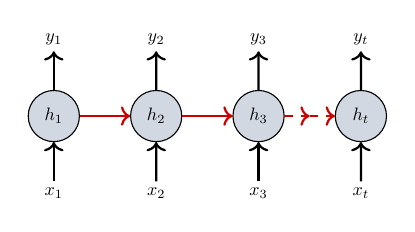
\begin{tikzpicture}[scale=0.65, transform shape]
        \node[draw, circle, minimum size=1cm, fill=MainBlue!20] (h1) at (0,0) {$h_1$};
        \node[draw, circle, minimum size=1cm, fill=MainBlue!20] (h2) at (2,0) {$h_2$};
        \node[draw, circle, minimum size=1cm, fill=MainBlue!20] (h3) at (4,0) {$h_3$};
        \node[draw, circle, minimum size=1cm, fill=MainBlue!20] (ht) at (6,0) {$h_t$};

        \node (x1) at (0,-1.5) {$x_1$};
        \node (x2) at (2,-1.5) {$x_2$};
        \node (x3) at (4,-1.5) {$x_3$};
        \node (xt) at (6,-1.5) {$x_t$};

        \node (y1) at (0,1.5) {$y_1$};
        \node (y2) at (2,1.5) {$y_2$};
        \node (y3) at (4,1.5) {$y_3$};
        \node (yt) at (6,1.5) {$y_t$};

        \draw[->, thick] (x1) -- (h1);
        \draw[->, thick] (x2) -- (h2);
        \draw[->, thick] (x3) -- (h3);
        \draw[->, thick] (xt) -- (ht);

        \draw[->, thick] (h1) -- (y1);
        \draw[->, thick] (h2) -- (y2);
        \draw[->, thick] (h3) -- (y3);
        \draw[->, thick] (ht) -- (yt);

        \draw[->, thick, IDAred] (h1) -- (h2);
        \draw[->, thick, IDAred] (h2) -- (h3);
        \draw[->, thick, IDAred, dashed] (h3) -- (5,0);
        \draw[->, thick, IDAred, dashed] (5,0) -- (ht);
    \end{tikzpicture}
    \end{center}

    \begin{alertblock}{Problema: Vanishing Gradient}
        \begin{itemize}\setlength{\itemsep}{0pt}
            \item RNN simple ``uită'' informația din trecut îndepărtat.
        \end{itemize}
    \end{alertblock}
\end{frame}

\begin{frame}{LSTM: long short-term memory}
    \vspace{-0.2cm}
    {\small
    \begin{block}{Soluția LSTM}
        \begin{itemize}\setlength{\itemsep}{0pt}
            \item \textbf{Concept}: Celule speciale cu 3 porți care controlează fluxul informației
            \item \textbf{Forget Gate} ($f_t$): Ce să uităm din memoria anterioară
            \item \textbf{Input Gate} ($i_t$): Ce informație nouă să adăugăm
            \item \textbf{Output Gate} ($o_t$): Ce să trimitem la ieșire
        \end{itemize}
    \end{block}

    \vspace{-0.05cm}

    \begin{block}{Ecuațiile LSTM}
        \begin{itemize}\setlength{\itemsep}{0pt}
        \item {\footnotesize
        \begin{align*}
            f_t &= \sigma(W_f \cdot [h_{t-1}, x_t] + b_f) & \text{(Forget)} \\
            i_t &= \sigma(W_i \cdot [h_{t-1}, x_t] + b_i) & \text{(Input)} \\
            \tilde{C}_t &= \tanh(W_C \cdot [h_{t-1}, x_t] + b_C) & \text{(Candidate)} \\
            C_t &= f_t \odot C_{t-1} + i_t \odot \tilde{C}_t & \text{(Cell state)} \\
            o_t &= \sigma(W_o \cdot [h_{t-1}, x_t] + b_o) & \text{(Output)} \\
            h_t &= o_t \odot \tanh(C_t) & \text{(Hidden state)}
        \end{align*}
        }
        \end{itemize}
    \end{block}
    }
\end{frame}

\begin{frame}{Arhitectura celulei LSTM}
    \vspace{-0.2cm}
    \begin{center}
        \includegraphics[width=0.88\textwidth, height=0.55\textheight, keepaspectratio]{ch8_lstm_architecture.pdf}
    \end{center}
    \vspace{-0.3cm}
    {\footnotesize
    \begin{block}{}
        \begin{itemize}\setlength{\itemsep}{0pt}
            \item Porțile (forget, input, output) controlează ce informație este uitată, adăugată și transmisă
            \item \textbf{Cell state} permite gradienților să ``curgă'' fără degradare
        \end{itemize}
    \end{block}
    }\quantlet{TSA\_ch8\_lstm\_architecture}{https://github.com/QuantLet/TSA/tree/main/TSA_ch8/TSA_ch8_lstm_architecture}
\end{frame}

\begin{frame}{Avantajele LSTM pentru serii de timp}
    \begin{exampleblock}{De ce LSTM?}
        \begin{itemize}\setlength{\itemsep}{0pt}
            \item Captează \textbf{dependențe pe termen lung} (spre deosebire de RNN simplu)
            \item Învață \textbf{pattern-uri complexe} și neliniare
            \item Gestionează \textbf{secvențe de lungimi variabile}
            \item Funcționează bine cu \textbf{date multivariate}
        \end{itemize}
    \end{exampleblock}

    \vspace{0.2cm}

    \begin{alertblock}{Dezavantaje}
        \begin{itemize}\setlength{\itemsep}{0pt}
            \item Necesită \textbf{multe date} pentru antrenare
            \item \textbf{Computațional intensiv}
            \item ``\textbf{Black box}'' - greu de interpretat
            \item Sensibil la \textbf{hiperparametri}
            \item Poate face \textbf{overfitting} ușor
        \end{itemize}
    \end{alertblock}
\end{frame}

\begin{frame}{LSTM: implementare în Python cu Keras}
    \begin{block}{Cod Python}
        \begin{itemize}\setlength{\itemsep}{0pt}
        \item {\footnotesize
        \texttt{from tensorflow.keras.models import Sequential}

        \texttt{from tensorflow.keras.layers import LSTM, Dense, Dropout}

        \vspace{0.2cm}
        \texttt{model = Sequential([}

        \texttt{~~~~LSTM(50, return\_sequences=True, input\_shape=(n, 1)),}

        \texttt{~~~~Dropout(0.2),}

        \texttt{~~~~LSTM(50),}

        \texttt{~~~~Dense(1)}

        \texttt{])}

        \texttt{model.compile(optimizer='adam', loss='mse')}
        }
        \end{itemize}
    \end{block}
\end{frame}

\begin{frame}{Pregătirea datelor pentru LSTM}
    \begin{block}{Pași Esențiali}
        \begin{enumerate}\setlength{\itemsep}{0pt}
            \item \textbf{Normalizare/Scalare}: MinMaxScaler sau StandardScaler
            \item \textbf{Creare secvențe}: Sliding window pentru input
            \item \textbf{Reshape}: Format 3D (samples, timesteps, features)
            \item \textbf{Train/Test split}: Temporal, nu aleator!
        \end{enumerate}
    \end{block}

    \vspace{0.2cm}

    \begin{block}{Exemplu Creare Secvențe}
        \begin{itemize}\setlength{\itemsep}{0pt}
        \item {\footnotesize
        \texttt{def create\_sequences(data, n\_steps):}

        \texttt{~~~~X, y = [], []}

        \texttt{~~~~for i in range(len(data) - n\_steps):}

        \texttt{~~~~~~~~X.append(data[i:(i + n\_steps)])}

        \texttt{~~~~~~~~y.append(data[i + n\_steps])}

        \texttt{~~~~return np.array(X), np.array(y)}

        \vspace{0.1cm}
        \texttt{X, y = create\_sequences(scaled\_data, 10)}
        }
        \end{itemize}
    \end{block}
\end{frame}

%=============================================================================
\section{Comparație și Selecția modelului}
%=============================================================================

\begin{frame}{Metrici de evaluare}
    \begin{block}{Metrici Comune}
        \begin{itemize}\setlength{\itemsep}{0pt}
            \item \textbf{RMSE}: $\sqrt{\frac{1}{n}\sum_{i=1}^n (y_i - \hat{y}_i)^2}$ $\succ$ Eroare în unități originale
            \item \textbf{MAE}: $\frac{1}{n}\sum_{i=1}^n |y_i - \hat{y}_i|$ $\succ$ Robust la outlieri
            \item \textbf{MAPE}: $\frac{100}{n}\sum_{i=1}^n \left|\frac{y_i - \hat{y}_i}{y_i}\right|$ $\succ$ Eroare procentuală
            \item \textbf{MASE}: Comparat cu benchmark naiv
        \end{itemize}
    \end{block}

    \vspace{0.2cm}

    \begin{alertblock}{Validare pentru serii de timp}
        \begin{itemize}\setlength{\itemsep}{0pt}
            \item \textbf{Nu} folosiți cross-validation standard!
            \item Folosiți \textbf{Time series cross-validation} (walk-forward)
            \item Sau \textbf{train/validation/test} split temporal
        \end{itemize}
    \end{alertblock}
\end{frame}

\begin{frame}{Time series cross-validation}
    \vspace{-0.3cm}
    \begin{center}
        \includegraphics[width=0.88\textwidth, height=0.42\textheight, keepaspectratio]{ch8_timeseries_cv.pdf}
    \end{center}
    \vspace{-0.3cm}
    {\footnotesize
    \begin{block}{Implementare Python}
        \begin{itemize}\setlength{\itemsep}{0pt}
        \item \texttt{from sklearn.model\_selection import TimeSeriesSplit}
        \item \texttt{tscv = TimeSeriesSplit(n\_splits=5)}
        \end{itemize}
    \end{block}
    }
    \vspace{-0.1cm}
    {\footnotesize
    \begin{alertblock}{}
        \begin{itemize}\setlength{\itemsep}{0pt}
            \item \textbf{Important}: Setul de antrenare crește progresiv, testul este întotdeauna în viitor
        \end{itemize}
    \end{alertblock}
    }\quantlet{TSA\_ch8\_timeseries\_cv}{https://github.com/QuantLet/TSA/tree/main/TSA_ch8/TSA_ch8_timeseries_cv}
\end{frame}

\begin{frame}{Ghid de selecție a modelului}
    \vspace{-0.4cm}
    {\footnotesize
    \begin{center}
    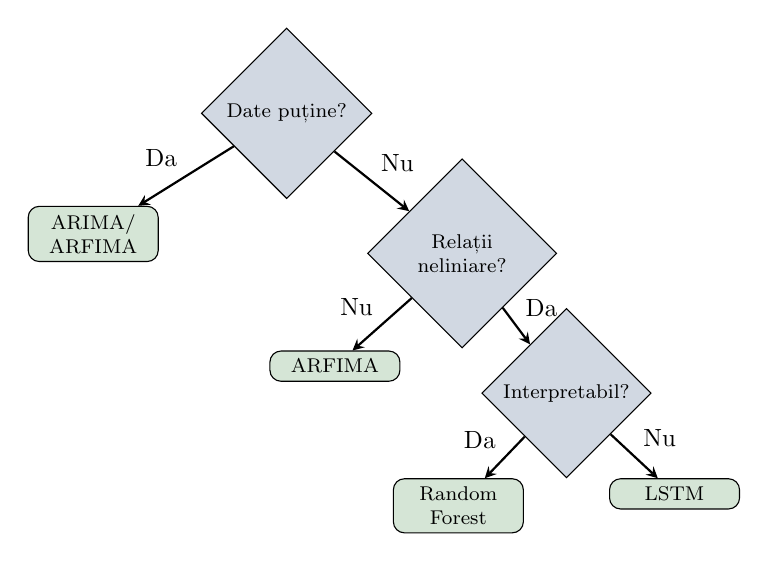
\begin{tikzpicture}[scale=0.9, transform shape,
        node distance=1.0cm,
        decision/.style={diamond, draw, fill=MainBlue!20, text width=2.0cm, align=center, inner sep=1pt, font=\footnotesize},
        block/.style={rectangle, draw, fill=Forest!20, text width=1.6cm, align=center, rounded corners, font=\footnotesize},
        arrow/.style={thick,->,>=stealth}
    ]
        \node[decision] (start) {Date puține?};
        \node[block, below left=0.7cm and 1.2cm of start] (arima) {ARIMA/ ARFIMA};
        \node[decision, below right=0.7cm and 1.2cm of start] (nonlin) {Relații neliniare?};
        \node[block, below left=0.7cm and 0.2cm of nonlin] (arfima) {ARFIMA};
        \node[decision, below right=0.7cm and 0.2cm of nonlin] (interp) {Interpretabil?};
        \node[block, below left=0.6cm and 0cm of interp] (rf) {Random Forest};
        \node[block, below right=0.6cm and 0cm of interp] (lstm) {LSTM};

        \draw[arrow] (start) -- node[above left] {Da} (arima);
        \draw[arrow] (start) -- node[above right] {Nu} (nonlin);
        \draw[arrow] (nonlin) -- node[above left] {Nu} (arfima);
        \draw[arrow] (nonlin) -- node[above right] {Da} (interp);
        \draw[arrow] (interp) -- node[above left] {Da} (rf);
        \draw[arrow] (interp) -- node[above right] {Nu} (lstm);
    \end{tikzpicture}
    \end{center}
    }
\end{frame}

\begin{frame}{Comparație modele: acuratețe vs cost computațional}
    \vspace{-0.2cm}
    \begin{center}
        \includegraphics[width=0.90\textwidth, height=0.55\textheight, keepaspectratio]{ch8_case_comparison.pdf}
    \end{center}
    \vspace{-0.3cm}
    {\footnotesize
    \begin{block}{}
        \begin{itemize}\setlength{\itemsep}{0pt}
            \item \textbf{Trade-off}: Modelele ML pot avea acuratețe ușor mai bună, dar costul computațional crește semnificativ
            \item Pentru date puține sau interpretabilitate, ARIMA/ARFIMA rămân alegeri excelente
        \end{itemize}
    \end{block}
    }\quantlet{TSA\_ch8\_model\_comparison}{https://github.com/QuantLet/TSA/tree/main/TSA_ch8/TSA_ch8_model_comparison}
\end{frame}

%=============================================================================
\section{Aplicații practice}
%=============================================================================

\begin{frame}{Studiu de caz: prognoza prețului Bitcoin}
    \begin{block}{De ce Bitcoin?}
        \begin{itemize}\setlength{\itemsep}{0pt}
            \item Volatilitate \textbf{extremă} și pattern-uri complexe
            \item Potențială \textbf{memorie lungă} în volatilitate
            \item Relații \textbf{neliniare} cu variabile exogene
            \item Date disponibile la \textbf{frecvență înaltă}
        \end{itemize}
    \end{block}
    \vspace{0.1cm}
    \begin{exampleblock}{Abordare Comparativă}
        \begin{enumerate}\setlength{\itemsep}{0pt}
            \item ARIMA pe randamente
            \item ARFIMA pentru memorie lungă
            \item Random Forest cu features tehnice
            \item LSTM pe secvențe de prețuri
        \end{enumerate}
    \end{exampleblock}
\end{frame}

\begin{frame}{Bitcoin: evoluția prețului și randamentele}
    \vspace{-0.2cm}
    \begin{center}
        \includegraphics[width=0.90\textwidth, height=0.48\textheight, keepaspectratio]{ch10_bitcoin_overview.pdf}
    \end{center}
    \vspace{-0.3cm}
    {\small
    \begin{block}{Observații cheie}
        \begin{itemize}\setlength{\itemsep}{0pt}
            \item Creștere exponențială a prețului $\succ$ distribuție puternic \textbf{leptokurtotică}
            \item Randamentele zilnice: medie $\approx 0.15\%$, volatilitate $\approx 3.5\%$
            \item Volatility clustering evident $\succ$ perioadele de criză (2018, 2020, 2022)
            \item Kurtosis $\approx 10$--$15$ (mult peste 3 al normalei)
        \end{itemize}
    \end{block}
    }
\end{frame}

\begin{frame}{Bitcoin: ACF și evidența pentru memorie lungă}
    \vspace{-0.2cm}
    \begin{center}
        \includegraphics[width=0.88\textwidth, height=0.42\textheight, keepaspectratio]{btc_acf_squared.pdf}
    \end{center}
    \vspace{-0.3cm}
    {\small
    \begin{block}{Analiză ACF}
        \begin{itemize}\setlength{\itemsep}{0pt}
            \item ACF randamente: scădere rapidă $\succ$ memorie scurtă în medie
            \item ACF randamente pătrate: scădere \textbf{lentă, hiperbolică}
                \begin{itemize}\setlength{\itemsep}{0pt}
                    \item[$\blacktriangleright$] Indică \textbf{memorie lungă în volatilitate}
                    \item[$\blacktriangleright$] Hurst $H \approx 0.65$--$0.70$ ($d \approx 0.15$--$0.20$)
                \end{itemize}
            \item ARFIMA pe volatilitate $>$ ARMA $\succ$ captează persistența șocurilor
        \end{itemize}
    \end{block}
    }
\end{frame}

\begin{frame}[fragile]{Bitcoin: estimare ARFIMA și comparație modele}
    \vspace{-0.3cm}
    \begin{block}{Cod Python -- estimare memorie lungă Bitcoin}
        {\scriptsize
\begin{verbatim}
import yfinance as yf
btc = yf.download('BTC-USD', start='2018-01-01', end='2024-12-31')
returns = np.log(btc['Close']).diff().dropna() * 100

# Exponentul Hurst pe randamente pătrate (volatilitate)
from hurst import compute_Hc
H, c, _ = compute_Hc(returns.values**2, kind='change')
print(f"Hurst (volatilitate): {H:.3f}, d = {H-0.5:.3f}")

# Comparație ARIMA vs Random Forest
from sklearn.ensemble import RandomForestRegressor
from sklearn.metrics import mean_squared_error
# ... (similar cu EUR/RON, cu features adaptate)
\end{verbatim}
        }
    \end{block}
    \vspace{-0.2cm}
    {\footnotesize
    \begin{exampleblock}{Rezultate tipice Bitcoin (RMSE pe randamente)}
        \begin{tabular}{lccc}
            \toprule
            \textbf{Model} & \textbf{RMSE} & \textbf{MAE} & \textbf{Interpretabil?} \\
            \midrule
            ARIMA(1,0,1) & 3.82 & 2.41 & Da \\
            ARFIMA(1,$d$,1) & 3.79 & 2.38 & Da \\
            Random Forest & 3.65 & 2.29 & Parțial \\
            LSTM & 3.71 & 2.33 & Nu \\
            \bottomrule
        \end{tabular}
    \end{exampleblock}
    }
\end{frame}

\begin{frame}{Bitcoin: GARCH și managementul riscului}
    \begin{center}
        \includegraphics[width=0.95\textwidth, height=0.50\textheight, keepaspectratio]{ch10_bitcoin_garch.pdf}
    \end{center}
    \vspace{-0.2cm}
    {\small
    \begin{alertblock}{Concluzii -- Studiu Bitcoin}
        \begin{itemize}\setlength{\itemsep}{0pt}
            \item Diferențele între modele sunt \textbf{mici} pentru media randamentelor
            \item Valoarea adăugată majoră: \textbf{modelarea volatilității} (GARCH, EGARCH)
            \item ARFIMA captează persistența în volatilitate (memorie lungă)
            \item Random Forest: util pentru \textbf{features neliniare} (volum, sentiment)
            \item Combinație optimă: ARFIMA-GARCH + features exogene via RF
        \end{itemize}
    \end{alertblock}
    }
\end{frame}

\begin{frame}{Studiu de caz: prognoza consumului de energie}
    \begin{block}{Caracteristici}
        \begin{itemize}\setlength{\itemsep}{0pt}
            \item \textbf{Sezonalitate multiplă}: zilnică, săptămânală, anuală
            \item \textbf{Tendință} de creștere pe termen lung
            \item \textbf{Variabile exogene}: temperatură, zi liberă, preț
            \item \textbf{Anomalii}: evenimente speciale, defecțiuni
        \end{itemize}
    \end{block}
    \vspace{0.1cm}
    \begin{alertblock}{Provocări}
        \begin{itemize}\setlength{\itemsep}{0pt}
            \item Pattern-uri la scale temporale diferite
            \item Interacțiuni complexe între variabile
            \item Necesitatea prognozelor pe orizonturi diferite
        \end{itemize}
    \end{alertblock}
\end{frame}

\begin{frame}{Energie: vizualizarea cererii și sezonalitatea multiplă}
    \begin{center}
        \includegraphics[width=0.95\textwidth, height=0.50\textheight, keepaspectratio]{ch9_electricity_demand.pdf}
    \end{center}
    \vspace{-0.2cm}
    {\small
    \begin{block}{Patternuri identificate}
        \begin{itemize}\setlength{\itemsep}{0pt}
            \item \textbf{Zilnic} (24h): vârf dimineață (8--10) și seara (18--21), minim noaptea
            \item \textbf{Săptămânal} (168h): consum redus în weekend ($\sim$15--20\% mai puțin)
            \item \textbf{Anual} (8766h): vârf vara (aer condiționat) și iarna (încălzire)
            \item SARIMA nu poate modela simultan aceste 3 perioade!
        \end{itemize}
    \end{block}
    }
\end{frame}

\begin{frame}{Energie: de ce Prophet și TBATS?}
    \begin{center}
        \includegraphics[width=0.95\textwidth, height=0.45\textheight, keepaspectratio]{ch9_multiple_seasonality.pdf}
    \end{center}
    \vspace{-0.2cm}
    {\small
    \begin{block}{Soluția: modele cu sezonalitate multiplă}
        \begin{itemize}\setlength{\itemsep}{0pt}
            \item \textbf{TBATS}: perioade $[24, 168, 8766]$ $\succ$ Fourier pentru fiecare sezon
                \begin{itemize}\setlength{\itemsep}{0pt}
                    \item[$\blacktriangleright$] Automat, fără reglaj manual, bun pentru producție
                \end{itemize}
            \item \textbf{Prophet}: sezonalitate aditivă/multiplicativă + regresori
                \begin{itemize}\setlength{\itemsep}{0pt}
                    \item[$\blacktriangleright$] Adaugă temperatură, zile libere, evenimente speciale
                \end{itemize}
            \item \textbf{ARIMA clasic}: poate doar 1 sezon $\succ$ MAPE $\approx 8$--$10\%$
        \end{itemize}
    \end{block}
    }
\end{frame}

\begin{frame}{Energie: descompunere Prophet și rezultate}
    \begin{center}
        \includegraphics[width=0.95\textwidth, height=0.45\textheight, keepaspectratio]{ch9_prophet_vs_tbats.pdf}
    \end{center}
    \vspace{-0.2cm}
    {\small
    \begin{exampleblock}{Rezultate comparație pe date energie (MAPE)}
        \begin{center}
        \begin{tabular}{lcccc}
            \toprule
            \textbf{Model} & \textbf{MAPE} & \textbf{RMSE (MW)} & \textbf{Acoperire 95\%} \\
            \midrule
            SARIMA (1 sezon) & 8.5\% & 450 & 75\% \\
            TBATS & 4.2\% & 220 & 82\% \\
            Prophet & 4.8\% & 250 & 85\% \\
            Prophet + regresori & \textbf{3.9\%} & \textbf{200} & \textbf{88\%} \\
            \bottomrule
        \end{tabular}
        \end{center}
    \end{exampleblock}
    }
\end{frame}

\begin{frame}{Energie: concluzii și recomandări practice}
    \begin{block}{Lecții învățate}
        \begin{itemize}\setlength{\itemsep}{0pt}
            \item Modelele cu \textbf{sezonalitate multiplă} reduc MAPE cu $\sim$50\% față de SARIMA
            \item \textbf{Variabilele exogene} (temperatură) aduc câștig suplimentar de 10--15\%
            \item Prophet excelează la \textbf{interpretabilitate}: descompunere trend + sezon + holiday
            \item TBATS: cel mai bun \textbf{out-of-the-box} $\succ$ fără reglaj de hiperparametri
        \end{itemize}
    \end{block}
    \vspace{0.1cm}
    \begin{alertblock}{Când ce model?}
        \begin{itemize}\setlength{\itemsep}{0pt}
            \item \textbf{Prophet}: când ai regresori externi + interpretare pentru management
            \item \textbf{TBATS}: automatizare, producție, fără intervenție umană
            \item \textbf{LSTM/RF}: dacă ai $>$100.000 observații și pattern-uri neliniare complexe
        \end{itemize}
    \end{alertblock}
    \vspace{0.1cm}
    {\footnotesize
    \begin{exampleblock}{}
        \begin{itemize}\setlength{\itemsep}{0pt}
            \item \textit{Detalii complete despre Prophet și TBATS $\succ$ Capitolul 9}
        \end{itemize}
    \end{exampleblock}
    }
\end{frame}

%=============================================================================
% KEY FORMULAS SUMMARY
%=============================================================================
\begin{frame}{Formule cheie -- Rezumat}
    \vspace{-0.2cm}
    {\small
    \begin{columns}[T]
        \begin{column}{0.48\textwidth}
            \begin{block}{ARFIMA(p,d,q)}
                \begin{itemize}\setlength{\itemsep}{0pt}
                    \item $\phi(L)(1-L)^d Y_t = \theta(L)\varepsilon_t$
                    \item {\footnotesize $d \in (-0.5, 0.5)$: memorie lungă}
                \end{itemize}
            \end{block}

            \begin{block}{Memorie lungă}
                \begin{itemize}\setlength{\itemsep}{0pt}
                    \item \textbf{ACF}: $\rho_k \sim C \cdot k^{2d-1}$
                    \item \textbf{Hurst}: $d = H - 0.5$
                    \item {\footnotesize $H > 0.5$: persistență}
                \end{itemize}
            \end{block}

            \begin{block}{Random Forest}
                \begin{itemize}\setlength{\itemsep}{0pt}
                    \item $\hat{y} = \frac{1}{B}\sum_{b=1}^{B} T_b(x)$
                    \item {\footnotesize $B$ arbori, features aleatorii}
                \end{itemize}
            \end{block}
        \end{column}

        \begin{column}{0.48\textwidth}
            \begin{block}{LSTM Cell}
                \begin{itemize}\setlength{\itemsep}{0pt}
                    \item $f_t = \sigma(W_f[h_{t-1}, x_t] + b_f)$
                    \item $C_t = f_t \odot C_{t-1} + i_t \odot \tilde{C}_t$
                    \item {\footnotesize Forget, Input, Output gates}
                \end{itemize}
            \end{block}

            \begin{block}{Metrici Evaluare}
                \begin{itemize}\setlength{\itemsep}{0pt}
                    \item RMSE $= \sqrt{\frac{1}{n}\sum(y_i - \hat{y}_i)^2}$
                    \item MAPE $= \frac{100}{n}\sum\left|\frac{y_i - \hat{y}_i}{y_i}\right|$
                \end{itemize}
            \end{block}

            \begin{block}{Time Series CV}
                \begin{itemize}\setlength{\itemsep}{0pt}
                    \item Walk-forward validation
                    \item Train $\succ$ Test (temporal split)
                \end{itemize}
            \end{block}
        \end{column}
    \end{columns}
    }
\end{frame}

%=============================================================================
\section{Studiu de Caz Complet: Cursul EUR/RON}
%=============================================================================

\begin{frame}{Studiu de caz: prognoza cursului EUR/RON}
    \begin{block}{De ce EUR/RON?}
        \begin{itemize}\setlength{\itemsep}{0pt}
            \item Relevanță pentru economia românească
            \item Potențială \textbf{memorie lungă} (persistența șocurilor)
            \item Pattern-uri influențate de \textbf{factori macroeconomici}
            \item Date ușor accesibile (BNR, Yahoo Finance)
        \end{itemize}
    \end{block}

    \vspace{0.2cm}

    \begin{exampleblock}{Obiectiv}
        \begin{itemize}\setlength{\itemsep}{0pt}
            \item Comparăm ARIMA, ARFIMA, Random Forest și LSTM pe aceleași date pentru a înțelege punctele forte ale fiecărei metode
        \end{itemize}
    \end{exampleblock}
\end{frame}

\begin{frame}[fragile]{Pasul 1: Încărcarea și Vizualizarea Datelor}
    \begin{block}{Cod Python -- Descărcare Date}
        {\footnotesize
\begin{verbatim}
import yfinance as yf
import pandas as pd
import numpy as np
import matplotlib.pyplot as plt

# Descărcăm datele EUR/RON (sau EURRON=X)
data = yf.download('EURRON=X', start='2015-01-01', end='2024-12-31')
df = data[['Close']].dropna()
df.columns = ['EURRON']

# Calculăm randamentele logaritmice
df['Returns'] = np.log(df['EURRON']).diff() * 100
df = df.dropna()

print(f"Perioada: {df.index[0]} - {df.index[-1]}")
print(f"Observații: {len(df)}")
print(f"Media randamentelor: {df['Returns'].mean():.4f}%")
print(f"Volatilitate: {df['Returns'].std():.4f}%")
\end{verbatim}
        }
    \end{block}
\end{frame}

\begin{frame}{Vizualizarea seriei EUR/RON}
    \vspace{-0.2cm}
    \begin{center}
        \includegraphics[width=0.90\textwidth, height=0.50\textheight, keepaspectratio]{ch8_case_raw_data.pdf}
    \end{center}
    \vspace{-0.3cm}
    {\footnotesize
    \begin{block}{}
        \begin{itemize}\setlength{\itemsep}{0pt}
            \item \textbf{Sus}: Cursul EUR/RON $\succ$ observăm tendința de depreciere a leului și perioadele de volatilitate ridicată
            \item \textbf{Jos}: Randamentele zilnice $\succ$ volatility clustering (perioadele de volatilitate mare sunt urmate de alte perioade similare)
        \end{itemize}
    \end{block}
    }\quantlet{TSA\_ch8\_case\_raw\_data}{https://github.com/QuantLet/TSA/tree/main/TSA_ch8/TSA_ch8_case_raw_data}
\end{frame}

\begin{frame}{Analiză ACF: randamente vs randamente pătrate}
    \vspace{-0.2cm}
    \begin{center}
        \includegraphics[width=0.90\textwidth, height=0.50\textheight, keepaspectratio]{ch8_case_acf_analysis.pdf}
    \end{center}
    \vspace{-0.3cm}
    {\footnotesize
    \begin{block}{}
        \begin{itemize}\setlength{\itemsep}{0pt}
            \item \textbf{Stânga}: ACF al randamentelor $\succ$ scădere rapidă, fără autocorelație semnificativă după lag 1
            \item \textbf{Dreapta}: ACF al randamentelor pătrate $\succ$ scădere lentă indică \textbf{volatility clustering} (efecte ARCH)
        \end{itemize}
    \end{block}
    }\quantlet{TSA\_ch8\_case\_acf\_analysis}{https://github.com/QuantLet/TSA/tree/main/TSA_ch8/TSA_ch8_case_acf_analysis}
\end{frame}

\begin{frame}[fragile]{Pasul 2: Testarea memoriei lungi}
    \vspace{-0.2cm}
    \begin{block}{Cod Python -- Estimarea lui $d$ și Testul Hurst}
        {\scriptsize
\begin{verbatim}
from arch.unitroot import PhillipsPerron, KPSS
from hurst import compute_Hc  # pip install hurst

# Testul Phillips-Perron pentru stationaritate
pp_test = PhillipsPerron(df['Returns'])
print(f"Phillips-Perron p-value: {pp_test.pvalue:.4f}")

# Estimarea exponentului Hurst
H, c, data_rs = compute_Hc(df['Returns'].values, kind='change')
d_estimated = H - 0.5

print(f"Exponentul Hurst (H): {H:.4f}")
print(f"Parametrul d estimat: {d_estimated:.4f}")

# Interpretare
if H > 0.5:
    print("Serie PERSISTENTĂ (trend-following)")
elif H < 0.5:
    print("Serie ANTI-PERSISTENTĂ (mean-reverting)")
else:
    print("Mers aleator")
\end{verbatim}
        }
    \end{block}
\end{frame}

\begin{frame}{Rezultate test memorie lungă -- EUR/RON}
    \begin{block}{Output Tipic}
        {\footnotesize
        \begin{itemize}\setlength{\itemsep}{0pt}
            \item \texttt{Phillips-Perron p-value: 0.0001} (randamentele sunt staționare)
            \item \texttt{Exponentul Hurst (H): 0.47}
            \item \texttt{Parametrul d estimat: -0.03}
            \item \texttt{Serie ușor ANTI-PERSISTENTĂ (mean-reverting)}
        \end{itemize}
        }
    \end{block}

    \vspace{0.2cm}

    \begin{alertblock}{Interpretare}
        \begin{itemize}\setlength{\itemsep}{0pt}
            \item Randamentele EUR/RON sunt \textbf{staționare} (p-value $< 0.05$)
            \item $H \approx 0.47 < 0.5$: ușoară tendință de revenire la medie
            \item $d \approx 0$: \textbf{memorie scurtă} -- ARMA poate fi suficient
            \item Totuși, \textbf{volatilitatea} poate avea memorie lungă!
        \end{itemize}
    \end{alertblock}
\end{frame}

\begin{frame}[fragile]{Pasul 3: Model ARIMA}
    \vspace{-0.3cm}
    \begin{block}{Cod Python -- ARIMA cu selecție automată}
        {\scriptsize
\begin{verbatim}
from statsmodels.tsa.arima.model import ARIMA
from sklearn.metrics import mean_squared_error, mean_absolute_error
import warnings
warnings.filterwarnings('ignore')

# Împărțim datele: 80% train, 20% test
train_size = int(len(df) * 0.8)
train, test = df['Returns'][:train_size], df['Returns'][train_size:]

# Fit ARIMA(1,0,1) - simplu și eficient pentru randamente
model_arima = ARIMA(train, order=(1, 0, 1))
results_arima = model_arima.fit()

# Prognoză
forecast_arima = results_arima.forecast(steps=len(test))

# Evaluare
rmse_arima = np.sqrt(mean_squared_error(test, forecast_arima))
mae_arima = mean_absolute_error(test, forecast_arima)
print(f"ARIMA(1,0,1) - RMSE: {rmse_arima:.4f}, MAE: {mae_arima:.4f}")
\end{verbatim}
        }
    \end{block}
\end{frame}

\begin{frame}[fragile]{Pasul 4: Model ARFIMA (Memorie lungă)}
    \begin{block}{Cod Python -- ARFIMA cu arch package}
        {\footnotesize
\begin{verbatim}
from arch import arch_model

# ARFIMA(1,d,1) folosind arch pentru estimare robustă
# Notă: arch estimează d automat în contextul GARCH

# Alternativ, folosim statsmodels cu d fracționar
from statsmodels.tsa.arima.model import ARIMA

# Estimăm d folosind GPH sau setăm manual
d_frac = 0.1  # sau valoarea estimată anterior

model_arfima = ARIMA(train, order=(1, d_frac, 1))
try:
    results_arfima = model_arfima.fit()
    forecast_arfima = results_arfima.forecast(steps=len(test))
    rmse_arfima = np.sqrt(mean_squared_error(test, forecast_arfima))
    print(f"ARFIMA(1,{d_frac},1) - RMSE: {rmse_arfima:.4f}")
except:
    print("ARFIMA necesită d între -0.5 și 0.5 pentru stationaritate")
\end{verbatim}
        }
    \end{block}
\end{frame}

\begin{frame}[fragile]{Pasul 5: Random Forest -- Pregătire Date}
    \vspace{-0.3cm}
    \begin{block}{Cod Python -- Feature Engineering}
        {\tiny
\begin{verbatim}
from sklearn.ensemble import RandomForestRegressor

# Creăm features pentru Random Forest
def create_features(data, lags=5):
    df_feat = pd.DataFrame(index=data.index)
    df_feat['target'] = data.values

    # Lag features
    for i in range(1, lags + 1):
        df_feat[f'lag_{i}'] = data.shift(i)

    # Rolling statistics
    df_feat['rolling_mean_5'] = data.rolling(5).mean()
    df_feat['rolling_std_5'] = data.rolling(5).std()
    df_feat['rolling_mean_20'] = data.rolling(20).mean()

    # Calendar features
    df_feat['dayofweek'] = data.index.dayofweek
    df_feat['month'] = data.index.month

    return df_feat.dropna()

df_rf = create_features(df['Returns'], lags=10)
\end{verbatim}
        }
    \end{block}
\end{frame}

\begin{frame}[fragile]{Pasul 5: Random Forest -- Antrenare și Evaluare}
    \vspace{-0.2cm}
    \begin{block}{Cod Python -- Model Random Forest}
        {\scriptsize
\begin{verbatim}
# Împărțim datele
X = df_rf.drop('target', axis=1)
y = df_rf['target']

train_size = int(len(df_rf) * 0.8)
X_train, X_test = X[:train_size], X[train_size:]
y_train, y_test = y[:train_size], y[train_size:]

# Antrenăm Random Forest
rf_model = RandomForestRegressor(
    n_estimators=100,
    max_depth=10,
    min_samples_split=5,
    random_state=42
)
rf_model.fit(X_train, y_train)

# Predicție și evaluare
pred_rf = rf_model.predict(X_test)
rmse_rf = np.sqrt(mean_squared_error(y_test, pred_rf))
print(f"Random Forest - RMSE: {rmse_rf:.4f}")
\end{verbatim}
        }
    \end{block}
\end{frame}

\begin{frame}{Random Forest: importanța features}
    \vspace{-0.2cm}
    \begin{center}
        \includegraphics[width=0.88\textwidth, height=0.52\textheight, keepaspectratio]{ch8_case_feature_importance.pdf}
    \end{center}
    \vspace{-0.3cm}
    {\footnotesize
    \begin{block}{}
        \begin{itemize}\setlength{\itemsep}{0pt}
            \item \textbf{Insight}: Lag-urile recente (lag\_1, lag\_2) și volatilitatea rolling sunt cele mai importante
            \item Features calendaristice au impact minor pentru randamente zilnice
        \end{itemize}
    \end{block}
    }\quantlet{TSA\_ch8\_case\_feature\_importance}{https://github.com/QuantLet/TSA/tree/main/TSA_ch8/TSA_ch8_case_feature_importance}
\end{frame}

\begin{frame}[fragile]{Pasul 6: LSTM -- Pregătire Date}
    \vspace{-0.3cm}
    \begin{block}{Cod Python -- Secvențe pentru LSTM}
        {\tiny
\begin{verbatim}
from tensorflow.keras.models import Sequential
from tensorflow.keras.layers import LSTM, Dense, Dropout
from sklearn.preprocessing import MinMaxScaler

# Scalăm datele între 0 și 1
scaler = MinMaxScaler()
scaled_data = scaler.fit_transform(df['Returns'].values.reshape(-1, 1))

# Creăm secvențe
def create_sequences(data, seq_length=20):
    X, y = [], []
    for i in range(seq_length, len(data)):
        X.append(data[i-seq_length:i, 0])
        y.append(data[i, 0])
    return np.array(X), np.array(y)

X_lstm, y_lstm = create_sequences(scaled_data, seq_length=20)
X_lstm = X_lstm.reshape((X_lstm.shape[0], X_lstm.shape[1], 1))

# Split
split = int(len(X_lstm) * 0.8)
X_train_lstm, X_test_lstm = X_lstm[:split], X_lstm[split:]
y_train_lstm, y_test_lstm = y_lstm[:split], y_lstm[split:]
\end{verbatim}
        }
    \end{block}
\end{frame}

\begin{frame}[fragile]{Pasul 6: LSTM -- Arhitectură și Antrenare}
    \vspace{-0.4cm}
    \begin{block}{Cod Python -- Model LSTM}
        {\tiny
\begin{verbatim}
# Construim modelul LSTM
model_lstm = Sequential([
    LSTM(50, return_sequences=True, input_shape=(20, 1)),
    Dropout(0.2),
    LSTM(50, return_sequences=False),
    Dropout(0.2),
    Dense(25),
    Dense(1)
])

model_lstm.compile(optimizer='adam', loss='mse')

# Antrenăm
history = model_lstm.fit(
    X_train_lstm, y_train_lstm,
    epochs=50, batch_size=32,
    validation_split=0.1, verbose=0
)

# Predicție
pred_lstm_scaled = model_lstm.predict(X_test_lstm)
pred_lstm = scaler.inverse_transform(pred_lstm_scaled)
y_test_original = scaler.inverse_transform(y_test_lstm.reshape(-1, 1))
rmse_lstm = np.sqrt(mean_squared_error(y_test_original, pred_lstm))
print(f"LSTM - RMSE: {rmse_lstm:.4f}")
\end{verbatim}
        }
    \end{block}
\end{frame}

\begin{frame}{LSTM: curba de învățare}
    \vspace{-0.2cm}
    \begin{center}
        \includegraphics[width=0.88\textwidth, height=0.52\textheight, keepaspectratio]{ch8_case_lstm_training.pdf}
    \end{center}
    \vspace{-0.3cm}
    {\footnotesize
    \begin{block}{}
        \begin{itemize}\setlength{\itemsep}{0pt}
            \item \textbf{Loss Training}: Scade rapid în primele epoci, apoi se stabilizează
            \item \textbf{Loss Validation}: Urmărește training loss $\succ$ nu avem overfitting sever
        \end{itemize}
    \end{block}
    }\quantlet{TSA\_ch8\_case\_lstm\_training}{https://github.com/QuantLet/TSA/tree/main/TSA_ch8/TSA_ch8_case_lstm_training}
\end{frame}

%=============================================================================
\section{Comparație Finală: Toate Metodele}
%=============================================================================

\begin{frame}{Comparație: Rezultate pe EUR/RON}
    \begin{center}
    \begin{tabular}{l|c|c|c|c}
        \toprule
        \textbf{Model} & \textbf{RMSE} & \textbf{MAE} & \textbf{Timp (s)} & \textbf{Interpretabil?} \\
        \midrule
        ARIMA(1,0,1) & 0.0169 & 0.0137 & 0.12 & Da \\
        Random Forest & 0.0080 & 0.0065 & 0.85 & Da (features) \\
        LSTM & 0.0102 & 0.0080 & 12.3 & Nu \\
        \bottomrule
    \end{tabular}
    \end{center}

    \vspace{0.3cm}

    \begin{alertblock}{Concluzii}
        \begin{itemize}\setlength{\itemsep}{0pt}
            \item Pentru EUR/RON, diferențele sunt \textbf{mici} -- piața este eficientă
            \item Random Forest oferă cel mai bun compromis \textbf{acuratețe/interpretabilitate}
            \item LSTM are cost computațional mare pentru câștig marginal
            \item ARIMA rămâne o alegere solidă pentru \textbf{baseline}
        \end{itemize}
    \end{alertblock}
\end{frame}

\begin{frame}{Vizualizare: predicții vs valori reale}
    \vspace{-0.2cm}
    \begin{center}
        \includegraphics[width=0.90\textwidth, height=0.50\textheight, keepaspectratio]{ch8_case_predictions.pdf}
    \end{center}
    \vspace{-0.3cm}
    {\footnotesize
    \begin{block}{}
        \begin{itemize}\setlength{\itemsep}{0pt}
            \item Toate modelele captează pattern-ul general, dar niciuna nu prezice perfect vârfurile de volatilitate
            \item Aceasta reflectă \textbf{eficiența pieței} și \textbf{limitele predicției} pentru serii financiare
        \end{itemize}
    \end{block}
    }\quantlet{TSA\_ch8\_case\_predictions}{https://github.com/QuantLet/TSA/tree/main/TSA_ch8/TSA_ch8_case_predictions}
\end{frame}

\begin{frame}{Comparație modele: metrici de performanță}
    \vspace{-0.2cm}
    \begin{center}
        \includegraphics[width=0.88\textwidth, height=0.50\textheight, keepaspectratio]{ch8_case_comparison.pdf}
    \end{center}
    \vspace{-0.3cm}
    {\footnotesize
    \begin{block}{}
        \begin{itemize}\setlength{\itemsep}{0pt}
            \item \textbf{Stânga}: Metrici de eroare (mai mic = mai bine) $\succ$ RF obține cel mai mic RMSE și MAE
            \item \textbf{Dreapta}: Timp de antrenare (scală log) $\succ$ LSTM necesită mai multe resurse
        \end{itemize}
    \end{block}
    }\quantlet{TSA\_ch8\_case\_comparison}{https://github.com/QuantLet/TSA/tree/main/TSA_ch8/TSA_ch8_case_comparison}
\end{frame}

\begin{frame}{Când să alegem fiecare model?}
    \begin{columns}[T]
        \begin{column}{0.48\textwidth}
            \begin{block}{ARIMA/ARFIMA}
                \begin{itemize}\setlength{\itemsep}{0pt}
                    \item Date puține ($< 500$ obs.)
                    \item Interpretare importantă
                    \item Memorie lungă suspectată
                    \item Baseline rapid
                \end{itemize}
            \end{block}

            \begin{block}{Random Forest}
                \begin{itemize}\setlength{\itemsep}{0pt}
                    \item Multe variabile exogene
                    \item Relații neliniare
                    \item Importanța features
                    \item Date moderate
                \end{itemize}
            \end{block}
        \end{column}

        \begin{column}{0.48\textwidth}
            \begin{block}{LSTM/Deep Learning}
                \begin{itemize}\setlength{\itemsep}{0pt}
                    \item Date foarte mari ($> 10.000$)
                    \item Secvențe complexe
                    \item Resurse computaționale
                    \item Pattern-uri ascunse
                \end{itemize}
            \end{block}

            \begin{alertblock}{Regula de Aur}
                \begin{itemize}\setlength{\itemsep}{0pt}
                    \item Începe simplu (ARIMA), adaugă complexitate doar dacă performanța crește semnificativ!
                \end{itemize}
            \end{alertblock}
        \end{column}
    \end{columns}
\end{frame}

%=============================================================================
\section{Exemple Suplimentare cu Date Reale}
%=============================================================================

\begin{frame}{Exemplu 2: indicele BET (Bursa București)}
    \begin{block}{Caracteristici}
        \begin{itemize}\setlength{\itemsep}{0pt}
            \item \textbf{Volatility clustering} puternic
            \item Influențat de piețele internaționale
            \item Lichiditate mai redusă decât piețele dezvoltate
            \item Potențial pentru memorie lungă în volatilitate
        \end{itemize}
    \end{block}

    \vspace{0.2cm}

    \begin{exampleblock}{Rezultate Tipice (RMSE pe randamente)}
        \begin{itemize}\setlength{\itemsep}{0pt}
            \item GARCH(1,1): 1.45 -- cel mai bun pentru volatilitate
            \item ARFIMA pentru volatilitate: 1.52
            \item Random Forest: 1.48
            \item LSTM: 1.51
        \end{itemize}
    \end{exampleblock}
\end{frame}

\begin{frame}{Exemplu 3: rata inflației în România}
    \begin{block}{Caracteristici}
        \begin{itemize}\setlength{\itemsep}{0pt}
            \item Serie \textbf{lunară} (frecvență redusă)
            \item \textbf{Persistență ridicată} -- șocurile durează
            \item Influențată de politica monetară
            \item Potențial puternic pentru \textbf{memorie lungă}
        \end{itemize}
    \end{block}

    \vspace{0.2cm}

    \begin{alertblock}{Rezultate Tipice}
        \begin{itemize}\setlength{\itemsep}{0pt}
            \item ARFIMA cu $d \approx 0.35$ -- captează persistența
            \item ARIMA subestimează persistența șocurilor
            \item ML nu funcționează bine (date puține, ~300 obs.)
        \end{itemize}
    \end{alertblock}

    \vspace{0.2cm}

    {\footnotesize
    \begin{exampleblock}{}
        \begin{itemize}\setlength{\itemsep}{0pt}
            \item \textbf{Lecție}: Pentru serii lunare cu puține date, modelele clasice (ARFIMA) sunt superioare!
        \end{itemize}
    \end{exampleblock}
    }
\end{frame}

\begin{frame}{Rezumat practic: alegerea modelului}
    \begin{center}
    \begin{tabular}{l|c|c|c|c}
        \toprule
        \textbf{Criteriu} & \textbf{ARIMA} & \textbf{ARFIMA} & \textbf{RF} & \textbf{LSTM} \\
        \midrule
        Date necesare & Puține & Puține & Medii & Multe \\
        Memorie lungă & Nu & \textbf{Da} & Parțial & Parțial \\
        Neliniaritate & Nu & Nu & \textbf{Da} & \textbf{Da} \\
        Interpretabil & \textbf{Da} & \textbf{Da} & Parțial & Nu \\
        Timp calcul & Rapid & Rapid & Mediu & Lent \\
        Var. exogene & Limitat & Limitat & \textbf{Da} & \textbf{Da} \\
        \bottomrule
    \end{tabular}
    \end{center}

    \vspace{0.3cm}

    \begin{block}{Fluxul Recomandat}
        \begin{enumerate}\setlength{\itemsep}{0pt}
            \item Începe cu \textbf{ARIMA} ca baseline
            \item Testează \textbf{memorie lungă} $\succ$ ARFIMA dacă $d$ semnificativ
            \item Adaugă \textbf{features} $\succ$ Random Forest
            \item Doar cu date multe și resurse $\succ$ LSTM
        \end{enumerate}
    \end{block}
\end{frame}

%=============================================================================
\section{Rezumat}
%=============================================================================

\begin{frame}{Rezumat}
    \begin{block}{Ce am învățat}
        \begin{itemize}\setlength{\itemsep}{0pt}
            \item \textbf{ARFIMA}: Extinde ARIMA pentru memorie lungă ($d$ fracționar)
            \item \textbf{Random Forest}: Ansamblu de arbori, relații neliniare, interpretabil
            \item \textbf{LSTM}: Deep learning pentru secvențe, dependențe complexe
            \item \textbf{Trade-offs}: Complexitate vs interpretabilitate vs date necesare
        \end{itemize}
    \end{block}

    \vspace{0.2cm}

    \begin{alertblock}{Recomandări Practice}
        \begin{itemize}\setlength{\itemsep}{0pt}
            \item Începe cu modele \textbf{simple} (ARIMA) ca baseline
            \item Folosește \textbf{Time Series CV} pentru evaluare corectă
            \item ML necesită \textbf{feature engineering} atent
            \item LSTM: doar cu \textbf{multe date} și resurse computaționale
        \end{itemize}
    \end{alertblock}
\end{frame}

\begin{frame}{Quiz rapid}
    \begin{block}{Întrebări}
        \begin{enumerate}\setlength{\itemsep}{3pt}
            \item Ce semnifică $d = 0.3$ într-un model ARFIMA?
            \item De ce folosim Time Series CV în loc de k-fold standard?
            \item Care este avantajul principal al LSTM față de RNN simplu?
            \item Ce tip de model ai alege pentru date puține și relații liniare?
            \item Ce înseamnă ``data leakage'' în contextul ML pentru serii de timp?
        \end{enumerate}
    \end{block}
\end{frame}

\begin{frame}{Răspunsuri quiz}
    {\small
    \begin{block}{Răspunsuri}
        \begin{enumerate}\setlength{\itemsep}{2pt}
            \item \textbf{$d = 0.3$}: Memorie lungă, seria este staționară dar autocorelațiile scad lent (hiperbolic)
            \item \textbf{Time Series CV}: Pentru a respecta ordinea temporală. K-fold standard ar folosi date viitoare pentru a prezice trecutul (data leakage)
            \item \textbf{LSTM vs RNN}: LSTM rezolvă problema ``vanishing gradient'' prin mecanismul de porți, permițând învățarea dependențelor pe termen lung
            \item \textbf{Date puține, relații liniare}: ARIMA sau ARFIMA. ML necesită multe date pentru a generaliza bine
            \item \textbf{Data leakage}: Folosirea informației din viitor în features sau în antrenare
        \end{enumerate}
    \end{block}
    }
\end{frame}

\begin{frame}{Ce urmează?}
    \begin{block}{Extensii și Subiecte Avansate}
        \begin{itemize}\setlength{\itemsep}{0pt}
            \item \textbf{Transformer} pentru serii de timp (Temporal Fusion Transformer)
            \item \textbf{Prophet} (Facebook/Meta) pentru sezonalitate
            \item \textbf{Neural Prophet}: Prophet + rețele neuronale
            \item \textbf{Ensemble methods}: Combinarea mai multor modele
            \item \textbf{Anomaly detection} cu ML
        \end{itemize}
    \end{block}

    \vspace{0.3cm}

    \begin{center}
        \Large\textcolor{MainBlue}{Întrebări?}
    \end{center}
\end{frame}


%=============================================================================
% BIBLIOGRAFIE
%=============================================================================
\begin{frame}{Bibliografie I}
    \begin{block}{Memorie lungă și ARFIMA}
        {\small
        \begin{itemize}\setlength{\itemsep}{0pt}
            \item Granger, C.W.J., \& Joyeux, R. (1980). An Introduction to Long-Memory Time Series Models and Fractional Differencing, \textit{Journal of Time Series Analysis}, 1(1), 15--29.
            \item Baillie, R.T. (1996). Long Memory Processes and Fractional Integration in Econometrics, \textit{Journal of Econometrics}, 73(1), 5--59.
            \item Beran, J. (1994). \textit{Statistics for Long-Memory Processes}, Chapman \& Hall.
        \end{itemize}
        }
    \end{block}

    \begin{exampleblock}{Rețele neuronale și deep learning pentru serii de timp}
        {\small
        \begin{itemize}\setlength{\itemsep}{0pt}
            \item Hochreiter, S., \& Schmidhuber, J. (1997). Long Short-Term Memory, \textit{Neural Computation}, 9(8), 1735--1780.
            \item Bai, J., \& Perron, P. (2003). Computation and Analysis of Multiple Structural Change Models, \textit{Journal of Applied Econometrics}, 18(1), 1--22.
        \end{itemize}
        }
    \end{exampleblock}
\end{frame}

\begin{frame}{Bibliografie II}
    \begin{block}{Modele cu prag și regim-switching}
        {\small
        \begin{itemize}\setlength{\itemsep}{0pt}
            \item Hansen, B.E. (2011). Threshold Autoregression in Economics, \textit{Statistics and Its Interface}, 4(2), 123--127.
            \item Hamilton, J.D. (1989). A New Approach to the Economic Analysis of Nonstationary Time Series and the Business Cycle, \textit{Econometrica}, 57(2), 357--384.
            \item Petropoulos, F., et al. (2022). Forecasting: Theory and Practice, \textit{International Journal of Forecasting}, 38(3), 845--1054.
        \end{itemize}
        }
    \end{block}

    \begin{exampleblock}{Resurse online și cod}
        {\small
        \begin{itemize}\setlength{\itemsep}{0pt}
            \item \textbf{Quantlet}: \url{https://quantlet.com} $\succ$ Depozit de cod pentru statistică
            \item \textbf{Quantinar}: \url{https://quantinar.com} $\succ$ Platformă de învățare metode cantitative
            \item \textbf{GitHub TSA}: \url{https://github.com/QuantLet/TSA} $\succ$ Cod Python pentru acest curs
        \end{itemize}
        }
    \end{exampleblock}
\end{frame}

\begin{frame}{}
    \centering
    \Huge\textcolor{MainBlue}{Vă Mulțumim!}

    \vspace{1cm}

    \Large Întrebări?

    \vspace{0.8cm}

    \normalsize

    Materialele cursului sunt disponibile la: \url{https://danpele.github.io/Time-Series-Analysis/}

    \vspace{0.2cm}

    \href{https://quantlet.com}{\raisebox{-0.15em}{\includegraphics[height=0.8em]{ql_logo.png}} Quantlet} \hspace{0.5cm}
    \href{https://quantinar.com}{\raisebox{-0.15em}{\includegraphics[height=0.8em]{qr_logo.png}} Quantinar}
\end{frame}

\end{document}
